%!TEX root = ../thesis.tex
\chapter{Methods}
\label{chap:methods}


\section{Synthetic aperture focusing technique (SAFT)}
\label{sec:SAFT}
The \ac{saft} is used to restore images from raw data of ultra sonic imaging techniques.
By combining the data of \acp{ascan} from a multitude of emitter-receiver combinations it is possible to reconstruct an high resolution image.

Figure \ref{ascan_example} shows the principle of an \ac{ascan}. The 3D-volume of the aperture is shown on the left side. For this example only two of the many transducers that normally are placed on the wall of the aperture are shown. On the right the plot of the pressure is shown by the graph. The actual \ac{ascan} consists of a discrete plot of the transition of the pressure at that receiving transducer where the pressure $p(t)$ is plotted over the time $t$. The first pulse in the graph is the transmission pulse that reaches the receiving transducer without much interaction of the pressure wave with matter. The second pulse originates after the first pressure wave scatters at a certain location in the tissue and has a lower amplitude than the first pulse. The amount of time it takes for the pulse to propagate from the emitter to the point of scattering and then to the receiving transducer is called \ac{tof}. The reason for the decreased amplitude of the reflected pulse compared to the transmission pulse is the longer path that the wave has to travel and as a consequence thereof the higher attenuation leads to the lower amplitude. 


\begin{figure}[H]
    \centering
    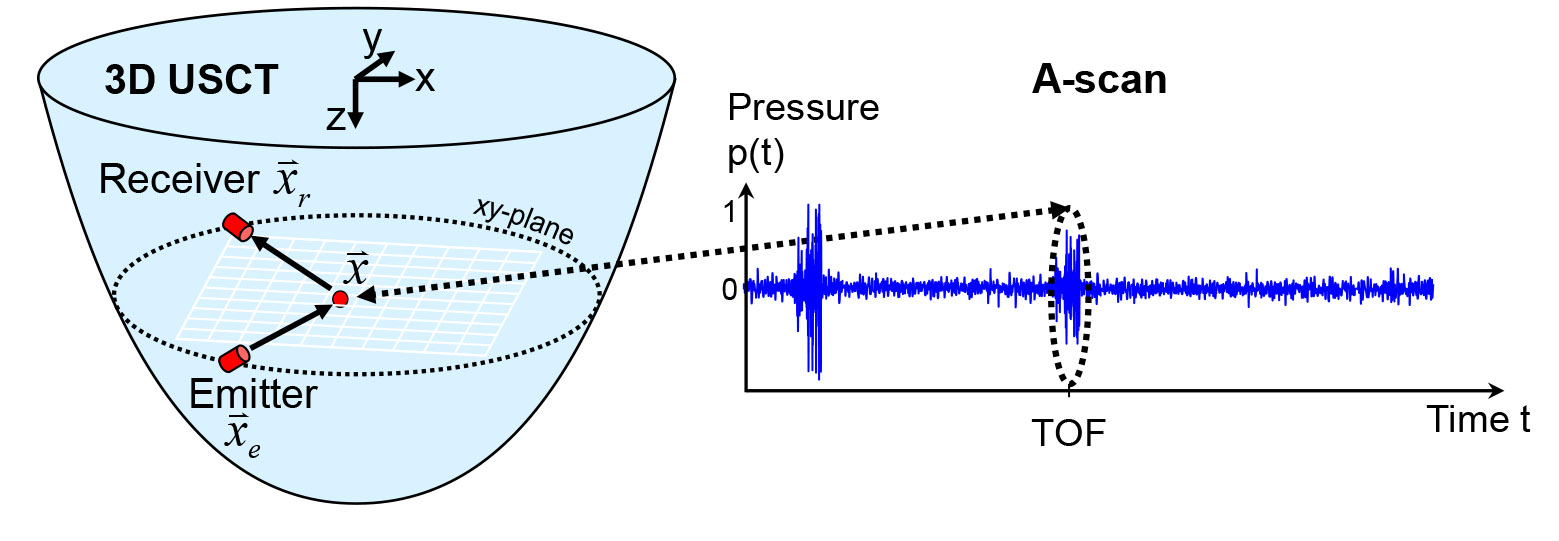
\includegraphics[width=1\textwidth]{GPU_based_3D_SAFT_reconstruction_including_phase_aberration-4.jpg}
    \caption{ Simple example of an \ac{ascan} for one emitter-reciever combination. One transducer $\overrightarrow{\chi_e}$ emits a pulsed wave-front into the aperture. The \ac{ascan} shows the pressure over the time measured by the receiving transducer $\overrightarrow{\chi_r}$. The first pulse in the diagram is the pulse cause by the transition of the emitted wave-front. The second pulse is from the reflection on an object in the aperture. Picture source: \cite{Kretzek2014GPUAberration}. }
    \label{ascan_example}
\end{figure}

There are two principal ways to reconstruct an image from a set of \acp{ascan} using the \ac{saft} which both yield quite a similar result but differ in the computation costs. Each voxel eventually gets assigned a certain value which corresponds to the intensity of that voxel in the final image. 

\bigskip

For the first method one starts with the desired voxel that the value should be calculated of.
A simple 2D-example of the xy-plane from figure \ref{ascan_example} is shown in figure \ref{SAFT_explain1}. On the left is the aperture with the 3D-volume shown as a 2D grid. The emitter $e_i$ and the two receiving transducers $r_j$ and $r_{j+1}$ are on the outer shell of the aperture. On the right two \acp{ascan} are depicted. The upper \ac{ascan} shows the plot of the pressure of the configuration where emitter $e_i$ transmits a wave-front and $r_j$ measures the transition of the pressure. The plot below is for emitter $e_i$ but this time with transducer $r_{i+1}$ receiving. Considering how close $r_j$ and $r_{j+1}$ are placed to each other in this example the \ac{ascan} on the bottom shows an rather exaggerated negative time shift compared to the \ac{ascan} above.

\begin{figure}[H]
    \centering
    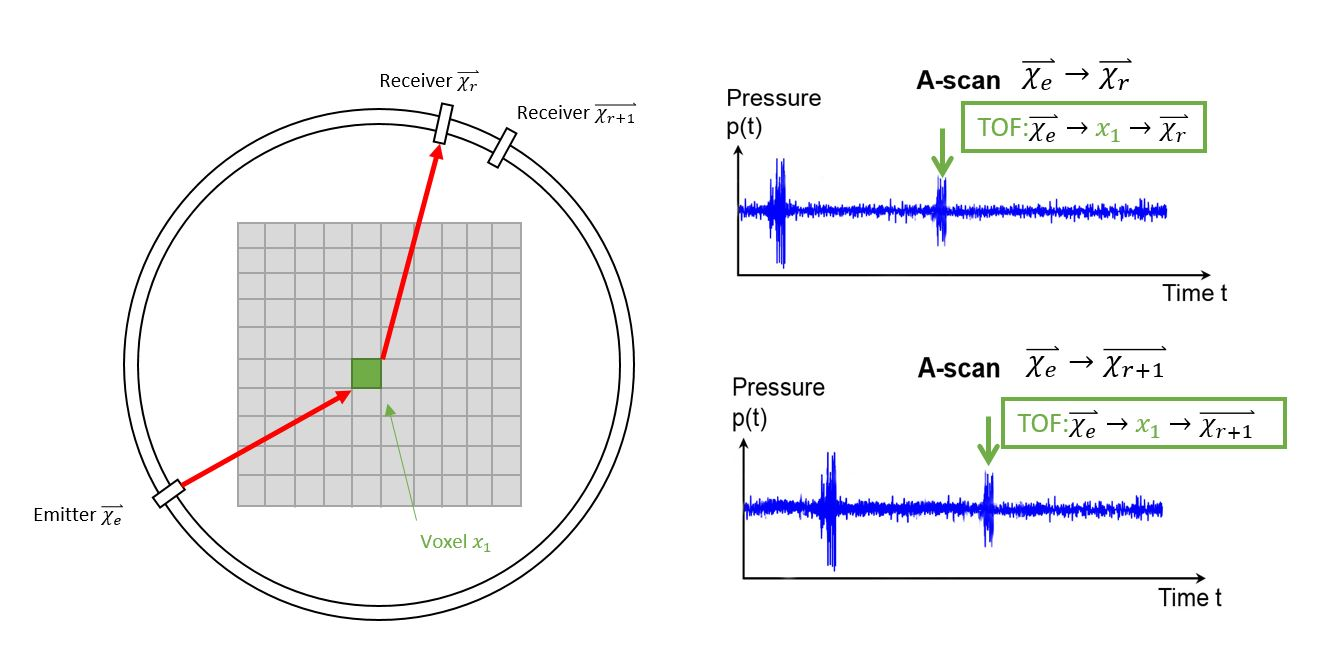
\includegraphics[width=1\textwidth]{SAFT_explaination1.jpg}
    \caption{Basic principle of the \ac{saft}. For one voxel every \ac{ascan} is analysed at a certain \ac{tof}. The final voxel value is the sum of every amplitude at the time in each corresponding \ac{ascan}. The procedure has to be repeated for each individual voxel. }
    \label{SAFT_explain1}
\end{figure}


If we know the location of our voxel in our plane then we can calculate the \ac{tof} from each emitter to each receiving transducer. For this basic example the equation \ref{eqation_tof} shows how to calculate the \ac{tof} for the first voxel when neglecting the different speeds of sound in for the different types of tissue.

\begin{equation}
TOF_{1,ij} =  \frac{dist_{e_i,x_1} + dist_{x_1,r_{j}} }{ SOS } 
\label{eqation_tof}
\end{equation}

$dist_{e_i,x_1}$ corresponds to the euclidean distance of the emitter $e_i$ to the desired voxel $x_1$ and $dist_{x_1,r_{j}}$ analogously to the euclidean distance from the voxel to the receiver.
The speed of the sound wave is considered by $SOS$ in the equation.

The \ac{tof} for the first emitter-receiver combination is shown a the green arrow in the upper \ac{ascan} in figure \ref{SAFT_explain1}. By accident the \ac{tof} is directly located at the peak of the reflected wave-front. To determine the corresponding sample in the discrete \ac{ascan} either a linear 1D-interpolation between the two samples left and right of the \ac{tof} can be performed. Otherwise a nearest neighbour interpolation can yield a viable time sample.
For this \ac{tof} the amplitude of the \ac{ascan} then is taken and added to the voxel value of voxel $x_1$. 
In the same manner the \ac{tof} of the second receiver-emitter configuration is calculated and a viable sample in the \ac{ascan} can be found. In this case the sample is not located at the peak of \ac{ascan} anymore. As well, for that time sample the value of the \ac{ascan} is added to the voxel value for $x_1$ even though it is considerably lower than before and does not influence the final voxel value that much. 
This procedure is repeated for every emitter-receiver combination and every aperture rotation shift so that the final result is the voxel value only for voxel $x_1$.
To reconstruct the whole 3D image these steps have to be repeated for every voxel in the volume.

Equation \ref{eqation_Voxel_value} shows the calculations necessary to get the voxel value $V_k$ for an arbitrary voxel $k$. 
\begin{equation}
V_k = \sum_{i}^{N_e}\sum_{j}^{N_r} A(TOF_{k,ij}) = \sum_{i}^{N}\sum_{j}^{N} \underset{ = TOF_{k,ij} } {\underbrace{\frac{ dist_{e_i,x_k} + dist_{x_k,r_{j}}}{SOS} }}
\label{eqation_Voxel_value}
\end{equation}

For $N$ transducers the reconstructed value $V$ of each voxel $k$ consists of the sum of each pressure values at the \ac{tof} in the respective \acp{ascan} for all emitter-receiver combinations ($N_e, N_r$). 

\bigskip

For the second possibility to reconstruct an image from the raw data we do not start at a certain voxel but look at each individual \ac{ascan}. In figure \ref{SAFT_explain2} the \ac{usct} aperture is shown this time with only one emitter-receiver configuration. On the right side the \ac{ascan} for this configuration is schematically plotted.

\begin{figure}[H]
    \centering
    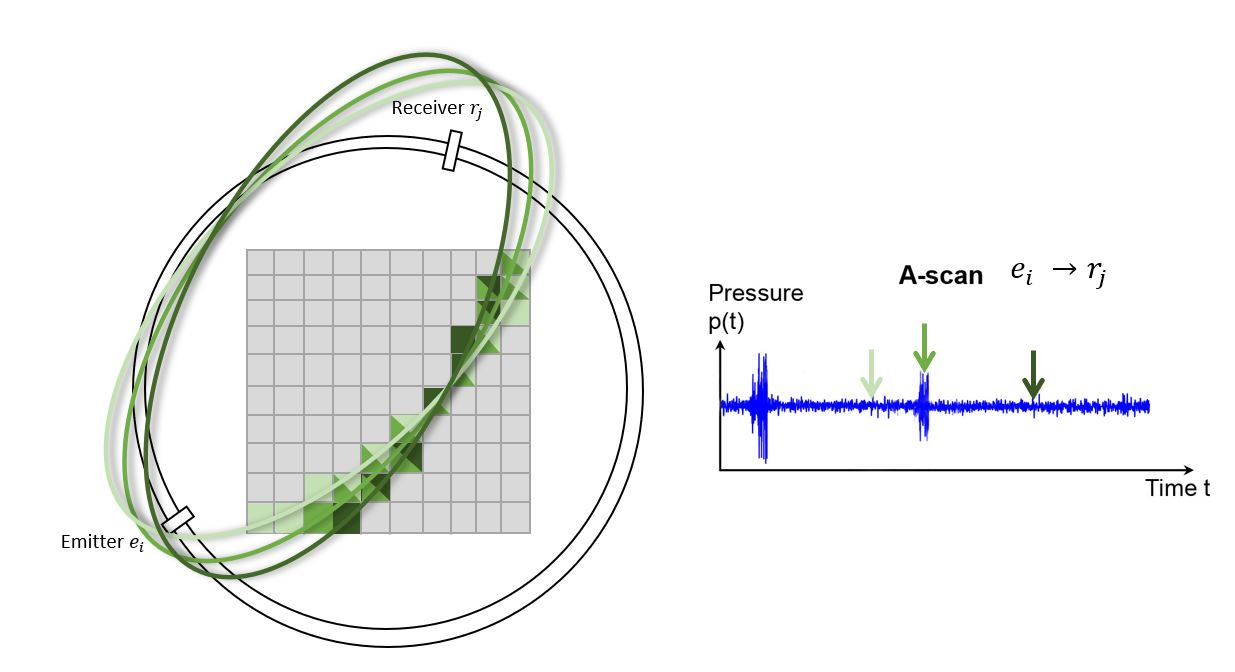
\includegraphics[width=1\textwidth]{SAFT_explaination2.jpg}
    \caption{ Alternative method to reconstruct the image for the \acp{ascan}. }
    \label{SAFT_explain2}
\end{figure}


In contrast to the first method we do not only pick one certain sample in the \ac{ascan} but a few. 
Theoretically one could use every sample in the \ac{ascan} to reconstruct the image, however is not recommendable as this would require a long time to compute. In general it is advisable to pick at least one sample at location of the maximum peak that is caused by the scattering of the wave front at the location of one voxel. In this example three samples are chosen marked by the arrows in the different shades of green. By choosing one sample in the \ac{ascan} we avoid having to interpolate during this step.
With these three chosen \acp{tof} in one \ac{ascan} and the location of the emitter and receiver it is not possible to determine only one voxel to add the amplitude values to. For one emitter-receiver combination and one certain \ac{tof} a multitude of voxels are eligible to be the source of the scattering. To be precise an eclipse covers every possible scattering location where the \ac{tof} from emitter $e_i$ to receiver $r_j$ is equal to the chosen \ac{tof} from the \ac{ascan}. For each of the three chosen \acp{tof} there is one eclipse in figure \ref{SAFT_explain2}. Along those eclipses to every voxel which is cut by the eclipse the amplitude value is added to. This is schematically shown by the different shapes of the squares beneath each eclipse. A single colour means, that to that voxel only one value was added. Analogously do two or even three colours indicate, that multiple pressure values are added to that voxels value. 
Bresenham's line drawing algorithm \cite{Bresenham2010AlgorithmPlotter} is used to decide which set of voxels approximates the eclipse best and therefore to which voxel the corresponding amplitude value is added. To find the suitable coordinates of each voxel an interpolation in 3D has to be performed.
This procedure leads to the fact, that many voxels get assigned pressure values even though they were not at the location of the scattering. However, when this procedure is repeated for every \ac{ascan} ultimately those voxels that are actually at the true location of the scattering will be part of so many eclipses that their final voxel value will be a lot higher than the surrounding noise. By superposing the voxel values the surrounding noise is negligible and does not affect the final image. An example is shown in figure \ref{eclipse_super}.


\begin{figure}[H]
    \centering
    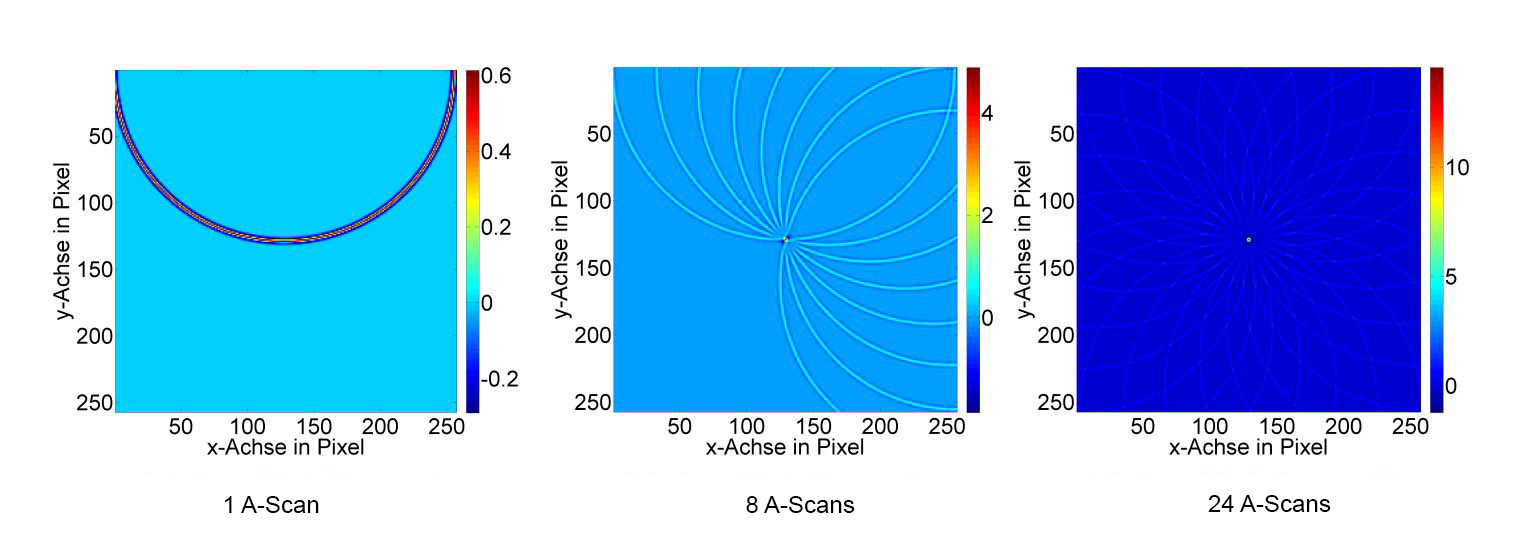
\includegraphics[width=1\textwidth]{eclipse_superposition_hucker.jpg}
    \caption{ Superposition of multiple eclipses during the reconstruction of the final image. By averaging the voxel values of multiple eclipses each eclipse loses significance in the final image.
    Source: \cite{PatrickHucker2014EvaluationRuckstreumodells}}
    \label{eclipse_super}
\end{figure}


For only one \ac{ascan} the value of only that one \ac{tof} of the \ac{ascan} is added to each voxel along the eclipse. Therefore, the eclipse is very prominent in the left-most pane of figure \ref{eclipse_super}. In the plot in the middle there are already eight different \acp{ascan} used. Each eclipse is still distinguishable but lost opacity nonetheless.
In the pane on the right side 24 \acp{ascan} are superimposed. At the point of the intersection of all 24 eclipses one single pixel has a rather high value whereas the surrounding eclipses are barely visible anymore. There more \acp{ascan} are used for the reconstruction the higher the contrast of the final image gets.

\bigskip

Both methods have their advantages and disadvantages. However, during this thesis the first reconstruction algorithm was used. One of the main reasons for that is that all the calculations are easily calculable in parallel and therefore profit from the high number of parallel threads on the GPU architecture. Furthermore, as was mentioned that the eclipse method makes multiple interpolations for each voxel in 3D necessary whereas the first method only interpolates in 1D between two sample values. So, by choosing the first method very expensive computation operations can be avoided.


Currently the reconstruction of a clinical relevant volume of 1024x64 voxels and 1.7 million of A-scans takes about 23 minutes \cite{Kretzek2014GPUAberration}.




\section{Segmentation of measurement volume}
In Section \ref{sec:SAFT} the \ac{saft} is explained. In that section it was assumed that each voxel receives one final voxel value $V_k$ which is independent of the direction of each emitter and receiver combination.
This assumption now is extended by a adding a further dimension to the output volume.











\section{Identification of faces}
For the analysis of the direction-dependent reflection characteristics each \ac{ascan} has to be assigned to a certain direction of the voxel.
Depending on which geometry was chosen for the segmentation of the volume there is a set of normals which are orthogonal to each face of the geometry. To assign a face to each \ac{ascan} it makes sense to calculate the angle $\angle (\overrightarrow{a},\overrightarrow{b})$ between the direction vector and each normal.


\begin{equation}
\centering
\angle (\overrightarrow{a},\overrightarrow{b}) = \varphi
\label{eqation_angle}
\end{equation}


\begin{equation}
\centering
cos(\varphi )  =   \frac{(\overrightarrow{a} \cdot \overrightarrow{b})}{\left \| \overrightarrow{a} \right \|_2  \cdot \left \| \overrightarrow{b} \right \|_2}
\label{eqation_cos_phi}
\end{equation}

\begin{equation}
\angle (\overrightarrow{a},\overrightarrow{b}) = 
cos^{-1} \left (  
\frac{(\overrightarrow{a} \cdot \overrightarrow{b})}{\left \| \overrightarrow{a} \right \|_2  \cdot \left \| \overrightarrow{b} \right \|_2} 
\right )
\label{eqation_angle_final}
\end{equation}

To identify the face which belongs to the corresponding \ac{ascan} the smallest angle of the set has to be found.

\qquad


\begin{gather*}
Centered
\end{gather*} 


For every emitter-receiver combination, for each voxel and each rotation position of the aperture one calculation of the angle between two vectors has to be performed. Depending on which geometry is used for every normal of the faces of the geometry this calculation hast to be repeated. The number of calculations results in:

\boxed{ \# Calculations = \#Voxel \cdot \#Emitter \cdot \#Receiver \cdot \#AperturRotation \cdot \#Faces}

For the case of using a 12 face dodecahedron, 628 emitters, 1413 receivers, only a single slice of 1024x64 voxels and ten aperture positions already $[628 \cdot 1413 \cdot 1024 \cdot 64 \cdot 10 \cdot 12] = 6.98x10^{12}$ calculations have to be  performed to find the smallest angle index. By decreasing the complexity of these calculations the performance of the reconstruction algorithm can be greatly improved. To reduce the computational cost it is not necessary to calculate the absolute angle between each vector combination. It simply can be proven that for certain circumstances one certain combination of direction vector and face-normal has the smallest angle of the available set. The following segment is adapted from \cite{PatrickHucker2014EvaluationRuckstreumodells} and some inaccuracies were corrected.

\qquad

In the following $\overrightarrow{v}$ is the direction vector from the \ac{ascan} which should be matched best to one of the norm vectors $\overrightarrow{n_i}$ from the $N$ faces of the used geometry.


\begin{equation}
\angle (\overrightarrow{v},\overrightarrow{n_i}) =  cos^{-1}\left (    \frac{(\overrightarrow{v} \cdot \overrightarrow{n_i})}{\left \| \overrightarrow{v} \right \|_2  \cdot {\left \| \overrightarrow{n_i} \right \|_2}}  \right ) 
\label{equation_with_v_n}
\end{equation}



For the first simplification we can neglect the $arccos$ in equation \ref{equation_with_v_n}. Since the arccosine is monotonically decreasing in the interval $[-1,1]$ (Figure \ref{accos_figure}) only the argument of the $arccos$ has to be regarded to find the smallest angle $\angle (\overrightarrow{v},\overrightarrow{n_i})$. To reach a small value for the arccosine function its argument has to become as big as possible.
\begin{equation}
min \left (  \angle (\overrightarrow{v},\overrightarrow{n_i}) \right ) =  max \left (    \frac{(\overrightarrow{v} \cdot \overrightarrow{n_i})}{\left \| \overrightarrow{v} \right \|_2  \cdot {\left \| \overrightarrow{n_i} \right \|_2}}  \right ) 
\label{equation_acos_neglect}
\end{equation}

\begin{figure}[H]
    \centering
    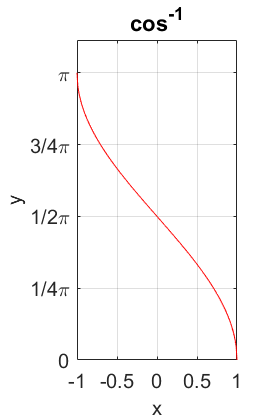
\includegraphics[width=0.3\textwidth]{accos.png}
    \caption{ Monotonically decreasing arccosine function.}
    \label{accos_figure}
\end{figure}

Since the euclidean norm of a normal vector $\left \| \overrightarrow{n_i} \right \|_2 = 1 , \forall i \in [1,...,N]$, the equation \ref{equation_acos_neglect} can be simplified further:


\begin{equation}
min \left (  \angle (\overrightarrow{v},\overrightarrow{n_i}) \right ) =  max \left (    \frac{(\overrightarrow{v} \cdot \overrightarrow{n_i})}{\left \| \overrightarrow{v} \right \|_2  \cdot { \underset{=1}{\underbrace{\left \| \overrightarrow{n_i} \right \|_2}}} }  \right ) = 
max \left (    \frac{(\overrightarrow{v} \cdot \overrightarrow{n_i})}{\left \| \overrightarrow{v} \right \|_2  }  \right )
\label{equation_acos_norm_simply}
\end{equation}

During the search of the smallest angle between the direction vector $\overrightarrow{v}$ and the set of normal vectors $\overrightarrow{n_i}$ the direction vector $\overrightarrow{v}$ does not change. 
The norm of the direction vector $\left \| \overrightarrow{v} \right \|_2$ is the same in every iteration of the search, thus has no influence on the final result and therefore can be remove from the formula.

\begin{equation}
min \left (  \angle (\overrightarrow{v},\overrightarrow{n_i}) \right ) = 
max \left (    \frac{(\overrightarrow{v} \cdot \overrightarrow{n_i})}{\left \| \overrightarrow{v} \right \|_2  }  \right ) = max \left (    \overrightarrow{v} \cdot \overrightarrow{n_i}  \right ) 
\label{equation_other_norm_simply}
\end{equation}

The final problem arises from equation \ref{equation_other_norm_simply}. The goal is to find the index $i_0$ for which the product of the direction vector $\overrightarrow{v}$ and the normal $\overrightarrow{n_{i_0}}$ is maximised: 

\begin{equation}
i_0 = \underset{i \in 0..N}{\mathrm{argmax}} \left (    \overrightarrow{v} \cdot \overrightarrow{n_i}  \right )
\label{equation_arg_max}
\end{equation}


\section{Performance evaluation}